\section{Background}
\label{sec:background}

\subsection{Cyber Physical and Real-Time Systems}
Cyber-Physical Systems (CPS) and Real-Time Systems (RTS) are digital systems that interact with the physical world. Examples of CPS include medical devices and systems, aerospace systems, autonomous vehicles, process control, and factory automation, building and environmental control and smart homes. These systems must operate dependably, safely, securely all in real-time. \cite{2010cps}.

Real-Time systems are designed to fulfill a specific set of functions and have tasks that come with varying degrees of strictness in terms of deadlines \cite{liu_rt}, from hard real-time systems like anti-lock braking systems on automobiles to soft real-time systems like an audio-video streaming system. These tasks generally have periodic repetitive loops, for example, a sensor periodically collects data from its surroundings, the system decides upon an action based on these inputs and sends appropriate commands to actuators. Hard real-time systems are designed to operate predictably and meet deadlines even under worst-case loads. The applications that run on these systems are known beforehand and are not modified online. This allows them to be profiled, tuned and certified before they are deployed.

As these systems are becoming more pervasive these days, security concerns for RTS and CPS are gaining importance given their implications in the physical realm \cite{karim2014cps_sec,2010cps}.

\subsection{System Causality Analysis}

A system event trace is a sequence of recorded interactions among multiple system objects (processes, files, network connections, etc.) \cite{XuCCS16}. These traces capture information flows in the system and can be used to reconstruct causal dependencies between events.

We represent information flows in the form of a dependency or provenance graph. System events are edges in the graph, annotated with metadata such as event timestamps. The nodes in the graph are typically processes and files. This representation is crucial for many forensic applications, such as root cause diagnosis, intrusion recovery, attack impact analysis and forward tracking, which perform causality tracking on the graph \cite{XuCCS16}. The tracking can be either in the forward or backward direction. Backward tracing involves tracing paths back from a given node to the source of the attack, while forward tracing involves following edges from a given node to identify the impact of an exploit. It is often difficult to perform such tracing in a server setting due to the problem of dependency explosion\cite{LeeZX13}.

The starting point for generating such graphs is auditing system-level events to capture event logs from the system. Linux Audit framework \cite{audit} is one of the most widely deployed auditing systems.

\subsection{Linux Audit Framework}
\begin{figure}[tbp]
    \centering
    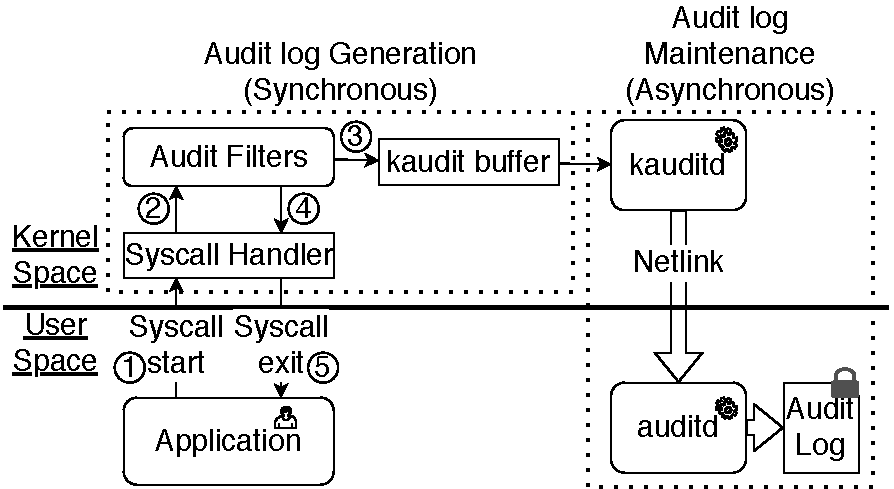
\includegraphics[width=\linewidth]{fig/audit_arch_2.pdf}
    \caption{\label{fig:audit_arch} Architecture of Linux Audit Framework. Audit logs are generated using auditing hooks in kernel's system call (Syscall) handler and temporarily stored in the kaudit buffer. Log maintenance is handled by two background daemons, kauditd and auditd.}
  \end{figure}

Linux Audit provides a way to track security-relevant information on a Linux based system. Based on user-configured rules, the audit system captures information about relevant events occurring in a system, most commonly in the form of system call logging. It is intended to be used for forensic analysis of mission-critical environments and determine violators of security policies along with the events which triggered the violations. \cite{audit}

The Audit system comprises of 2 sub-systems: the user-space applications and utilities, and the system call processing unit in kernel-space, as shown in Figure \ref{fig:audit-arch}. The system administrator specifies the audit rules and configurations using the Audit control utility \texttt{auditctl} and enables the system to be audited. The system call processing unit hooks into each system call invocation and filters relevant calls based on the configured rules. On intercepting these events, they are enriched with useful information like the executable name, the effective user id, inode information for files, etc and are queued onto a kernel buffer in a FIFO manner. A kernel thread \texttt{kauditd} reads these events and passes them onto the user-space daemon \texttt{auditd} over a netlink socket connection. \texttt{auditd} further ensures that these events are logged to disk successfully and are available for reporting and analysis via userspace tools like \texttt{aureport} and \texttt{ausearch}.
